\label{sec:evsel_paper}

We apply several other selection criteria to minimize instrumental 
background and electronic noise. In particular,
accepted events must have at least one good primary vertex
(Section~\ref{sec:reconstruction}). 
Backgrounds from additional beam interactions 
are reduced by applying a variety of requirements on charged tracks.
Finally, calorimeter noise is minimized through restrictions on
timing and electronic pulse shapes expected for signals. 


Dijet events are required to have at least two AK7 jets, each with
$\pt > 50$ \GeV and $|y| < 2.5$, 
and each jet must satisfy the jet quality criteria discussed in
Ref.~\cite{particleflow}.
No third-jet veto is applied. 

Reconstruction of \PW\ and \Z\ bosons in V+jet events 
begins with identification of charged leptons and a
calculation of $\met$, described in the previous 
section. 
Candidates for $\Z\to\ell^+\ell^-$ ($\ell=e$ or $\mu$) decays are reconstructed by combining 
two isolated electrons or muons and requiring the dilepton invariant 
mass to be in the $80<M_{\ell\ell}<100\GeV$ range.  
An accurate measurement of $\met$ is essential for distinguishing
the W signal from background processes.
The $\met$ in the event is defined using the PF objects,
and this analysis requires $\met > 50\GeV$.
Candidate $\WtoLN_\ell$ decays are identified primarily through the presence of 
a significant $\met$ and a single isolated lepton of large $\pt$, with
\pt and \mtW\ of the \PW\ candidate obtained by combining the lepton 
and the $\met$ vectors.

The analysis of V+jet events is mainly of interest for the 
regime of $\pt^{\mathrm{V}}> 120$ GeV, in which the opposing jet tends to have large $\pt$ as well, because of momentum conservation.
In fact, the leading jet in each event (independent of clustering 
algorithm and jet radius) is required to have $\pt > 125\GeV$ and $|y| < 2.5$.
A back-to-back topology between the vector boson and the leading jet 
is ensured by the additional selection of $\Delta \phi(\mathrm{V},\rm{jet})>2$ and 
$\Delta R (\ell,\rm{jet})>1$. 
Requiring such highly boosted jets, in addition to the tight isolation  
criteria for the leptons, greatly suppresses the background from multijet production.
In the $\WtoLN_\ell$+jet analysis, additional rejection 
of multijet background is achieved by requiring 
%$\met>$ 50 GeV and
$m_\mathrm{T}(\PW) > 50\GeV$.
No subleading-jet veto is applied. 

Figures~\ref{fig:Vjetpt}(a) and (b) show the $\pt$ distributions
for the leading AK7 jet selected in Z+jet and W+jet candidate events,
respectively. 
Given the unique signature for highly-boosted vector 
bosons recoiling from jets, the selections suffice to define very pure samples of V+jet events. 
In the $\Z(\ell\ell)$+jet analysis, the additional
constraint on dilepton mass removes almost all
background contributions, yielding a purity of ${\approx} 99\%$ for {\Z}$+$jet events, with
${\approx} 1\%$ contamination from diboson production.
The \PW+jet candidate sample contains ${\approx} 82\%$ \PW+jet events, 
with small background contributions from $\mathrm{t\bar{t}}$ (13\%), 
single top-quark (3\%), and diboson and {\Z}$+$jet (1\% each) events based on MC simulation.
%In the \Z$(\ell\ell)$+jet analysis, the additional 
%constraint on the dilepton mass removes almost all 
%background contributions, yielding a purity of about 99\% for \Z+jet events, with 
%1\% contamination from diboson production. 
The small number of events expected from these processes are 
subtracted using MC predictions for the jet mass 
from the \PW+jet candidate events,  
before correcting the data for detector effects.
Similarly, the small number of events expected from diboson production
are subtracted from the \Z+jet candidates.  

\begin{figure}[htbp]
\centering
%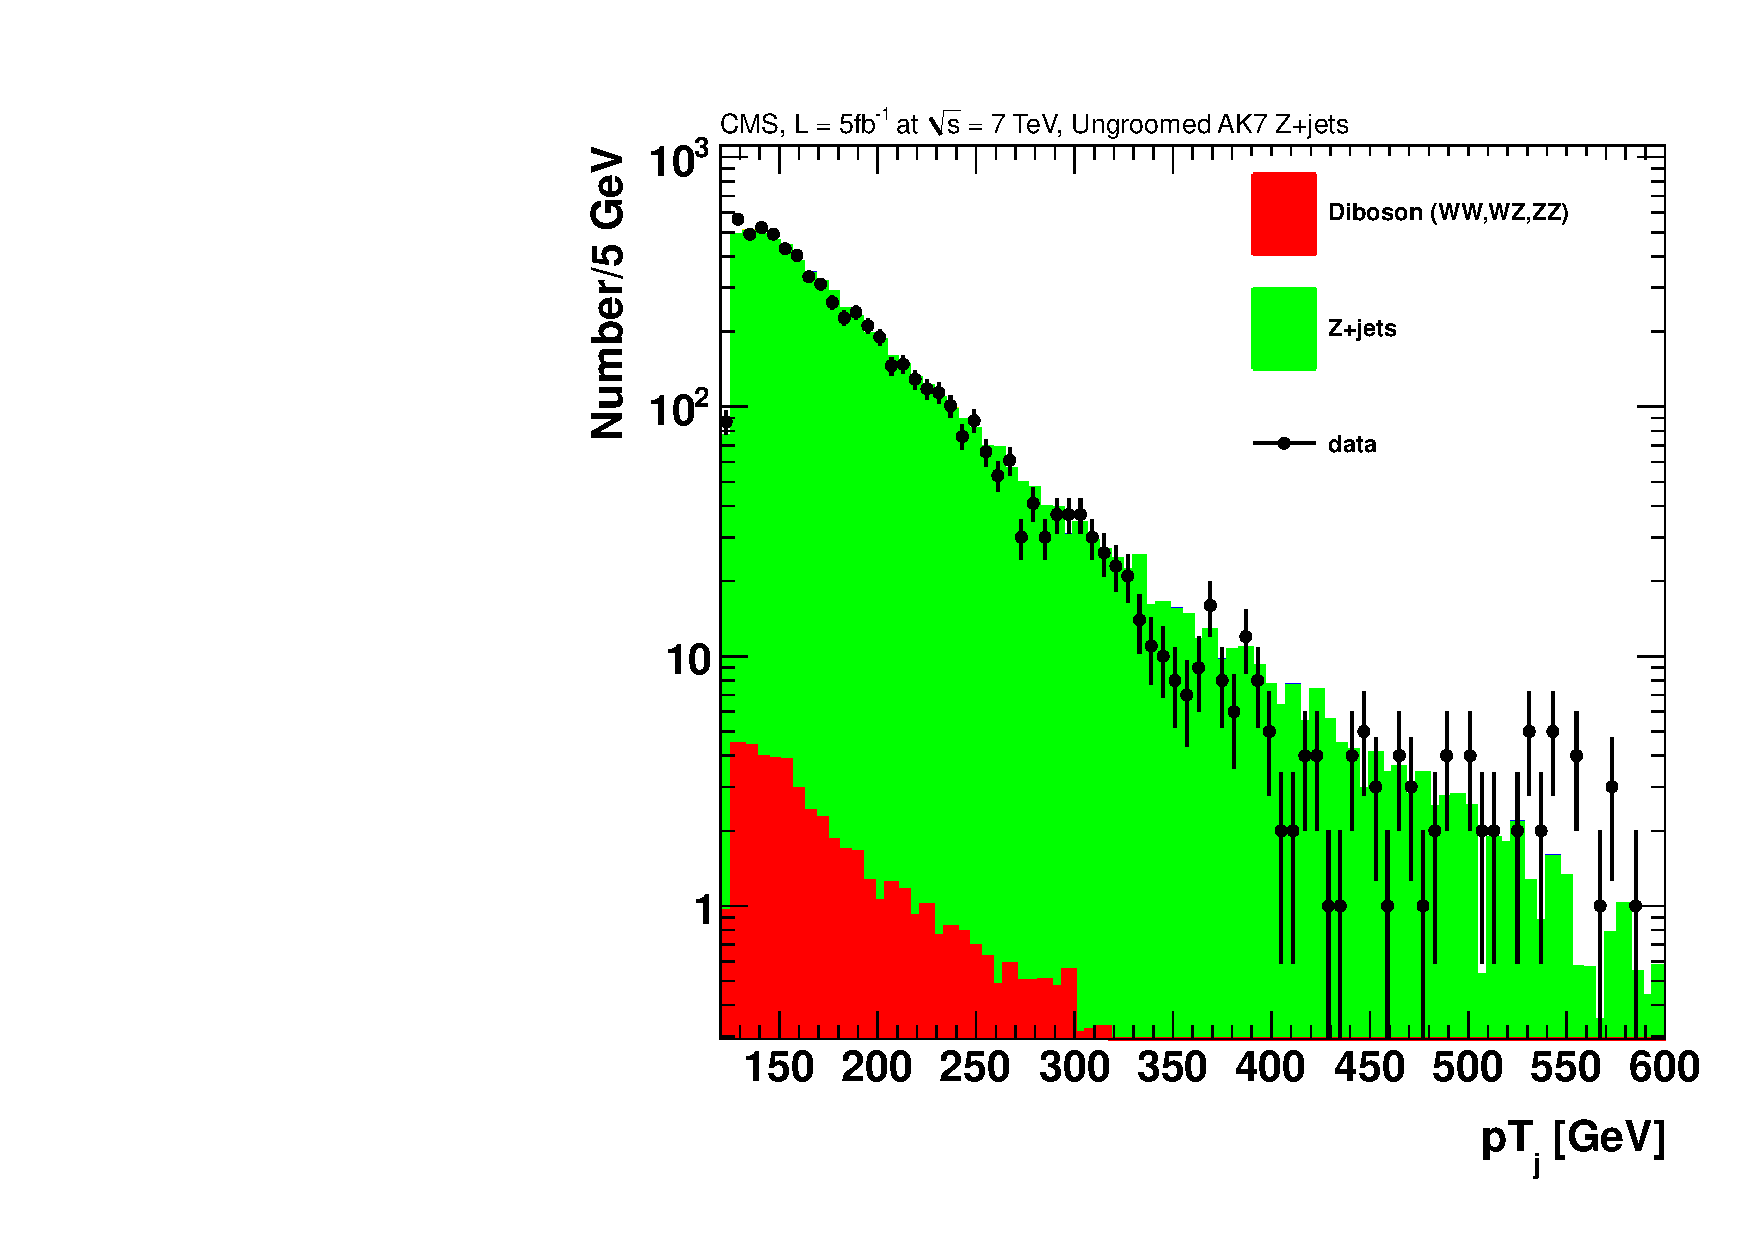
\includegraphics[width=0.495\textwidth]{figs/jetptZ_ak7.pdf}
%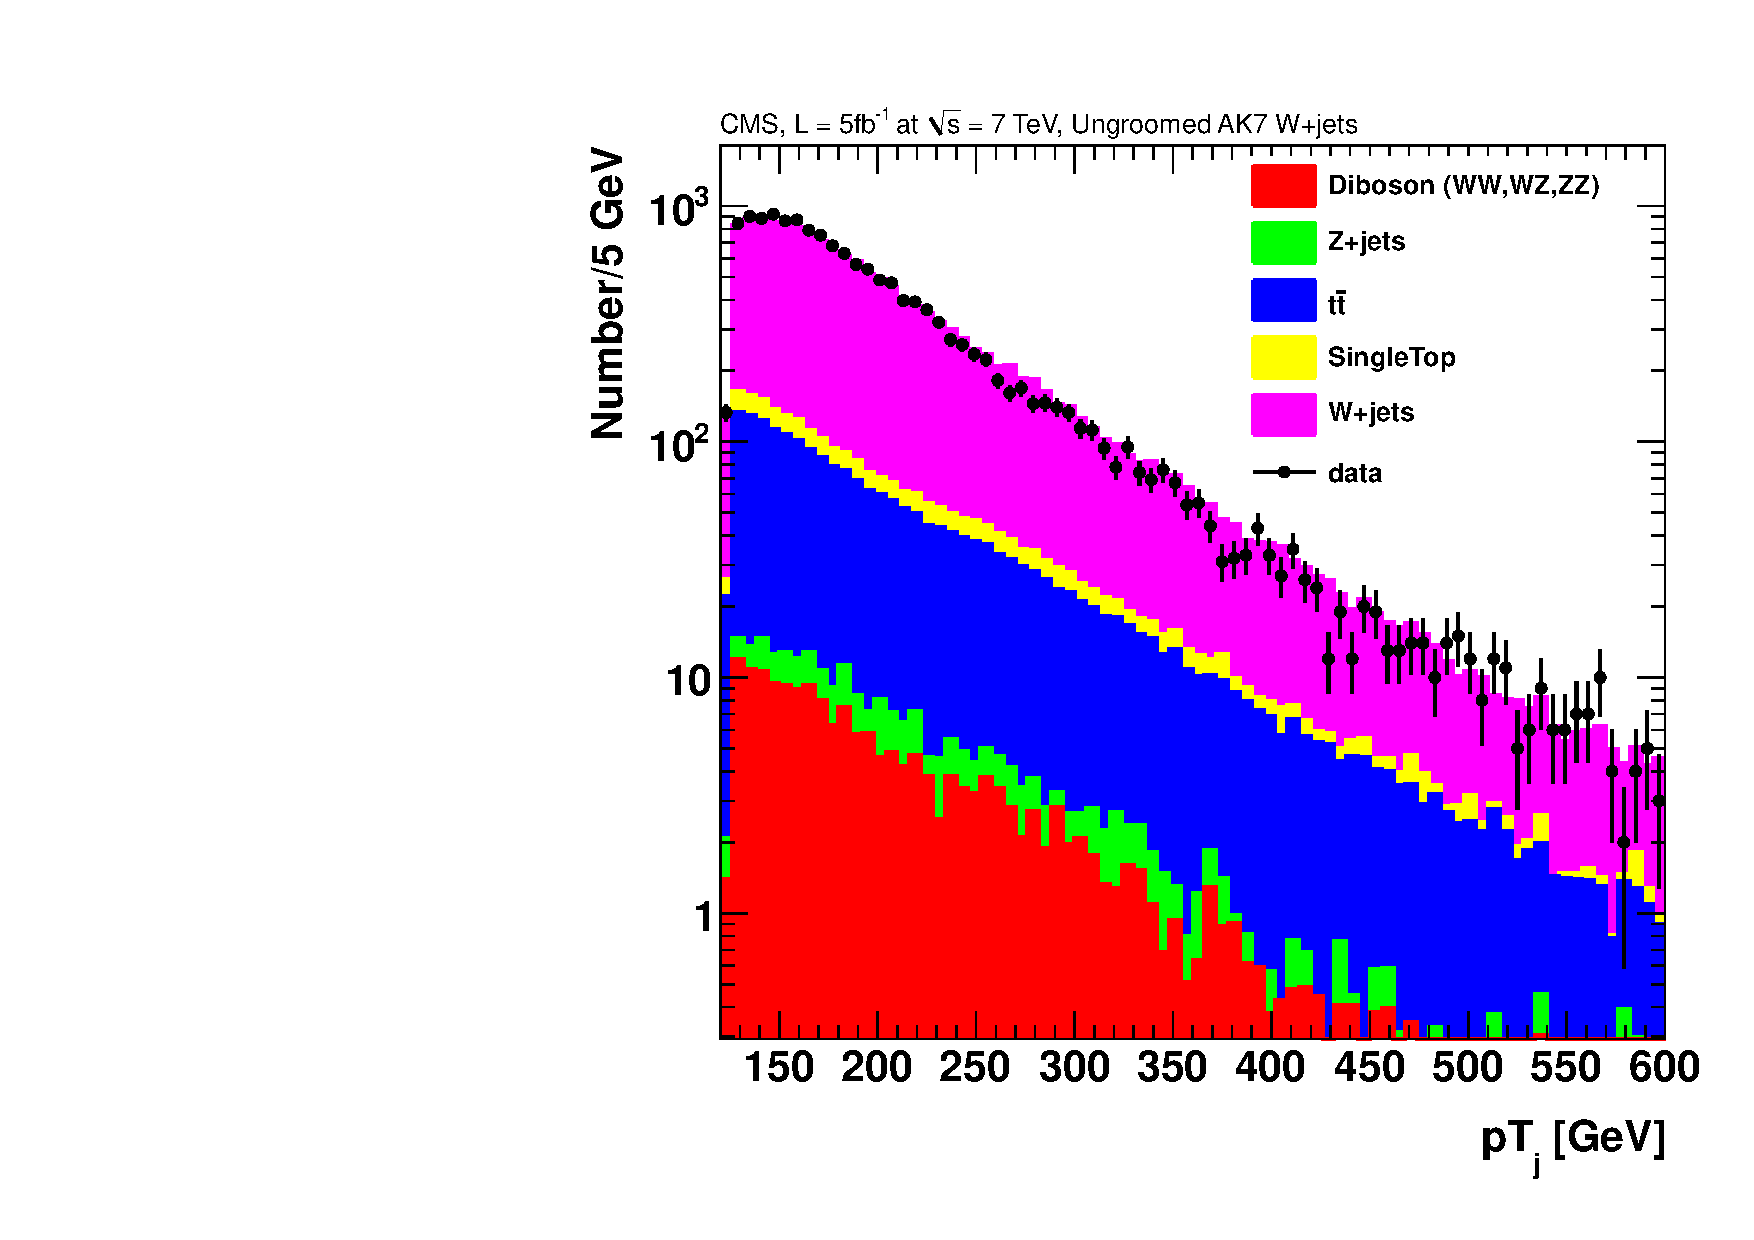
\includegraphics[width=0.495\textwidth]{figs/jetptW_ak7.pdf}
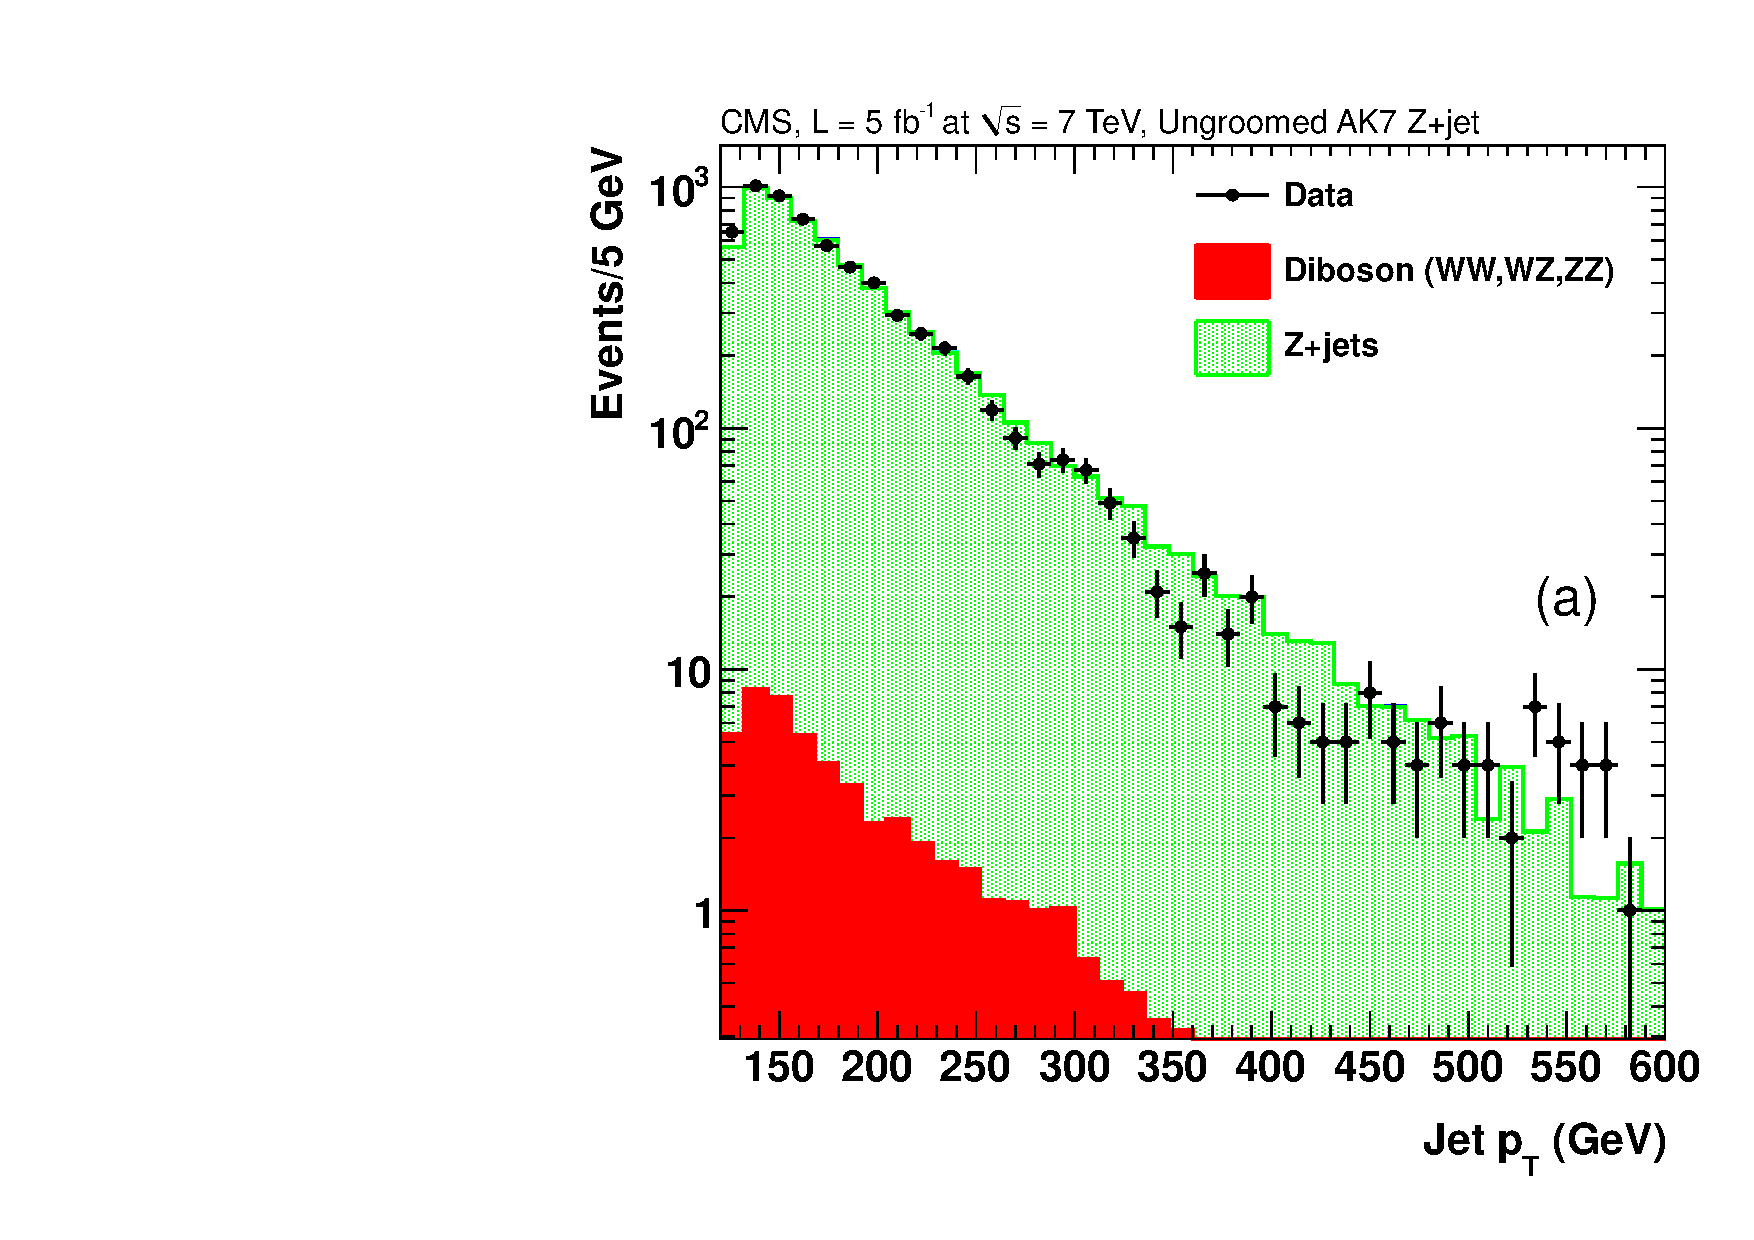
\includegraphics[width=0.495\textwidth]{figs/jetpt_ak7_Zmm.pdf}
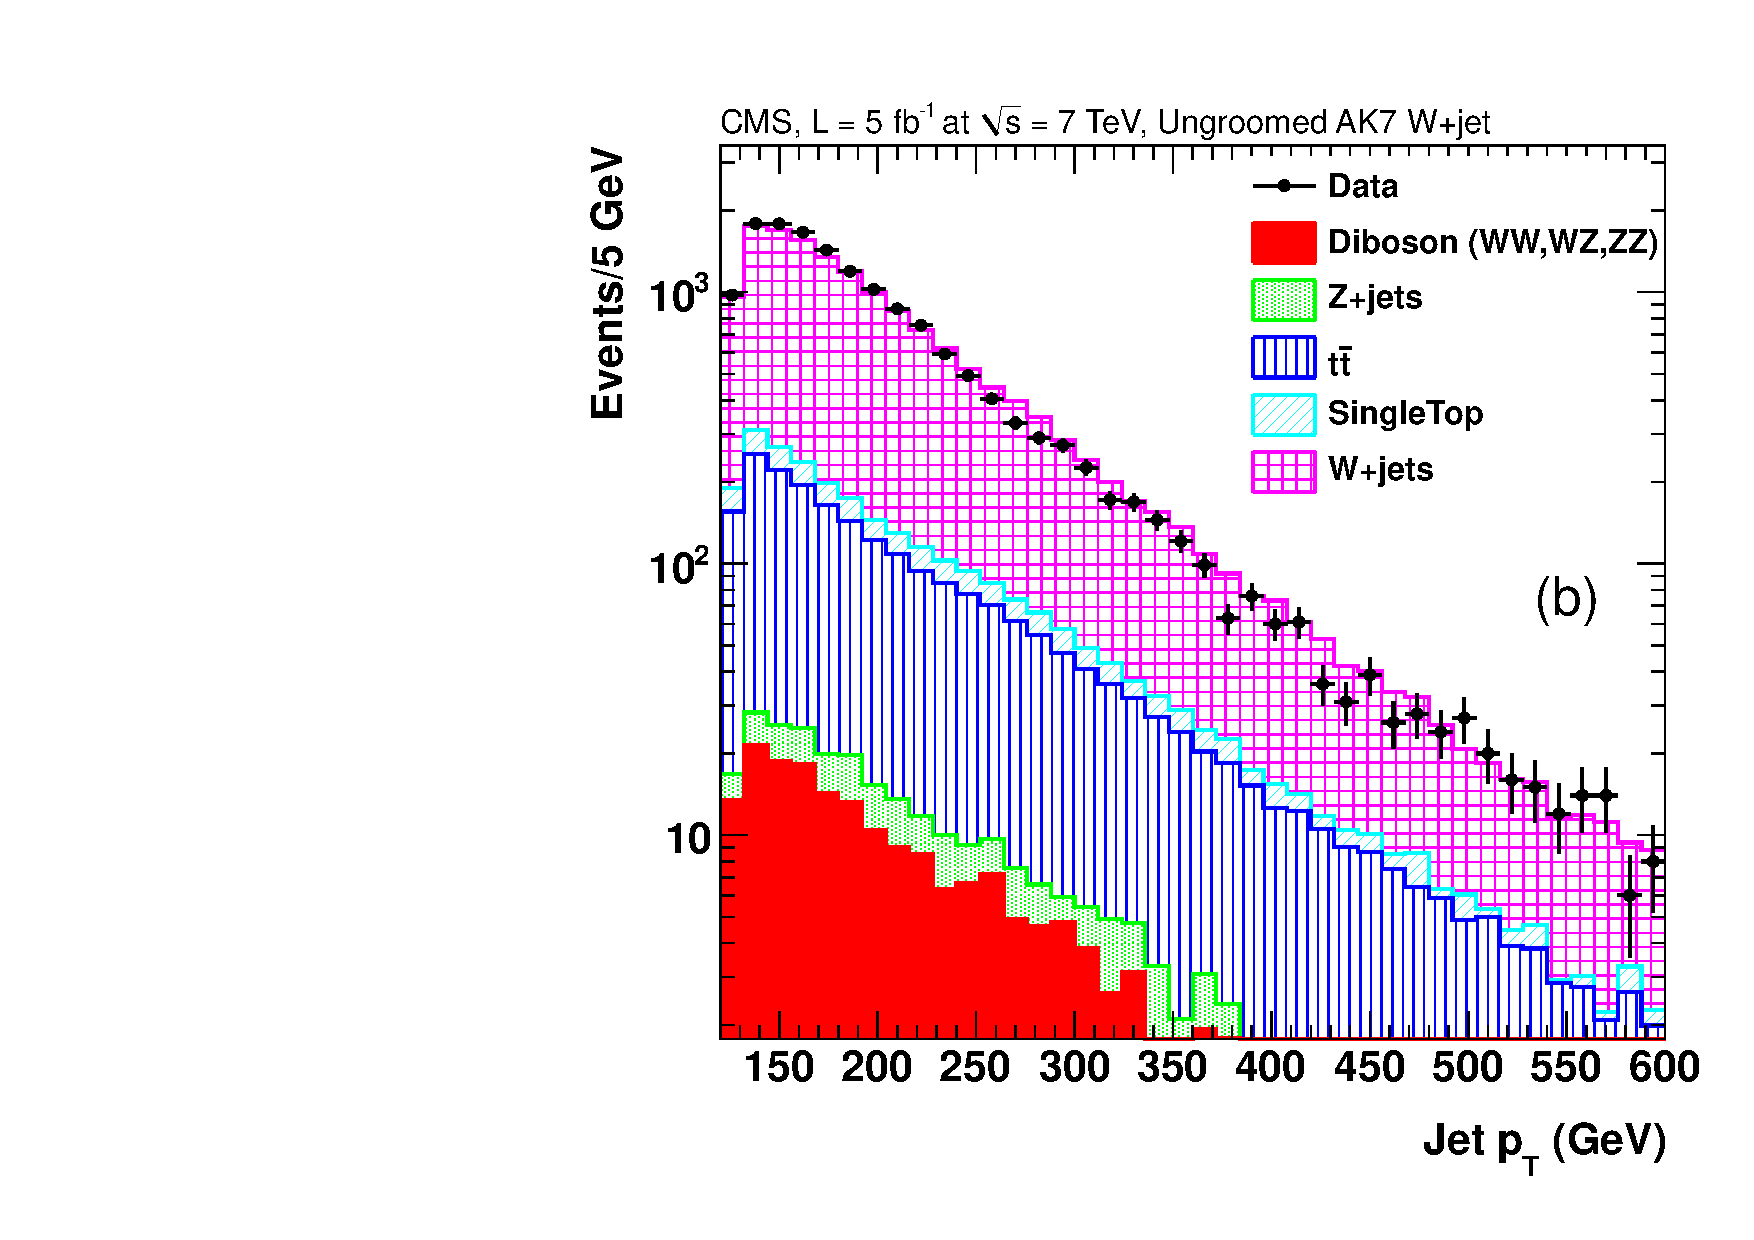
\includegraphics[width=0.495\textwidth]{figs/jetpt_ak7_Wenu.pdf}
\caption{The $\pt$ distribution for the leading AK7 jet in accepted (a)~\cPZ+jet and (b)~\PW+jet events.
\label{fig:Vjetpt}}
\end{figure}
